\chapter{功和能}

\begin{introduction}
	\item \nameref{3.1}
	\item \nameref{3.2}
	\item \nameref{3.3}
	\item \nameref{3.4}
	\item \nameref{3.5}
	\item \nameref{3.6}
\end{introduction}

\section{功} \label{3.1}

\subsection{恒力做功}

\begin{equation}
	A = Fs \cos \theta \label{C3-eq1}
\end{equation}

写成矢量点积的形式为

\begin{equation}
	A = \va*{F} \cdot \va*{s} \label{C3-eq2}
\end{equation}

\subsection{变力做功}

\textbf{力$\va*{F}$在路程$ab$上的功$A$, 等于力$\va*{F}$在路程$ab$的各段上所有元功的和. }

取元功

\begin{equation*}
	\dd{A} = \va*{F} \cdot \dd{\va*{r}} 
\end{equation*}

也可以写为

\begin{equation*}
	\dd{A} = F \dd{s} \cos \theta
\end{equation*} 

两端取积分, 得变力$\va*{F}$做功

\begin{equation}
	A = \int_{a(L)}^{b} \va*{F} \dd{\va*{r}} = \int_{a(L)}^{b} F \cos \theta \dd{s} \label{C3-eq3}
\end{equation}

\begin{note}
	上式为第二型线积分, 详见《工科数学分析基础(第三版)》第六章第七节“第二型线积分”部分. 
\end{note}

在直角坐标系中

\begin{equation}
	A = \int_{a(L)}^{b} \qty(F_x \dd{x} + F_y \dd{y} + F_z \dd{z}) \label{C3-eq4}
\end{equation}

上式表明, \textbf{当几个力同时作用在质点上时, 这些力在某一过程中分别对质点所做功的总和, 等于这些力的合力在同一过程中对质点所做的功. }

\subsection{功率}

\begin{definition}[功率] \label{C3-df1}
	
	{\heiti 功率} 是力在单位时间内所做的功. 
	
	平均功率
	
	\begin{equation}
		\overline{P} = \dfrac{\Delta A}{\Delta t} \label{C3-eq5}
	\end{equation}

    瞬时功率
    
    \begin{equation}
    	P = \lim\limits_{\Delta t \to 0} \dfrac{\Delta A}{\Delta t} = \dv{A}{t} \label{C3-eq6}
    \end{equation}

    由于$\dd{A} = \va*{F} \cdot \dd{\va*{r}}$, 则上式可以写成
    
    \begin{equation}
    	P = \dfrac{\va*{F} \cdot \dd{\va*{r}}}{\dd{t}} = \va*{F} \cdot \va*{v} = F v \cos \theta \label{C3-eq7}
    \end{equation}
    
\end{definition}

式(\ref{C3-eq7})表明, \textbf{瞬时功率等于力沿力作用点速度方向的投影和速度大小的乘积, 或者说瞬时功率等于力矢量与力作用点的速度矢量的点乘积. }

\section{几种常见力的功} \label{3.2}

\begin{enumerate}
	
	\item 重力的功
	
	\begin{equation}
		A = mg (z_1 - z_2) \label{C3-eq8}
	\end{equation}
	
	重力所做的功等于重力的大小乘以质点起始位置与终末位置的高度差. 
	
	\item 万有引力的功
	
	\begin{equation}
		A = GMm \qty(\dfrac{1}{r_2} - \dfrac{1}{r_1}) \label{C3-eq9}
	\end{equation}
	
	\item 弹性力的功(弹簧弹力的功)
	
	\begin{equation}
		A = \dfrac{1}{2}kx_1^2 - \dfrac{1}{2}kx_2^2 \label{C3-eq10}
	\end{equation}
	
	作用于质点的弹性力所做的功, 等于弹簧劲度系数乘以质点始、末位置弹簧变形量平方之差的一半. 
	
	\item 摩擦力的功
	
	\begin{equation}
		A = - \mu mgs \label{C3-eq11}
	\end{equation}
	
\end{enumerate}

\newpage

\section{动能定理} \label{3.3}

\subsection{质点动能定理}

\begin{theorem}[质点动能定理] \label{C3-th1}
	
	微分形式
	
	\begin{equation}
		\dd{A} = \dd{\qty(\dfrac{1}{2} m v^2)} \label{C3-eq12}
	\end{equation}
	
	上式表明, 质点动能的微分, 等于作用于质点的合力的元功. 
	
	\vskip 0.3cm
		
	积分形式(路径$M_1M_2$上)
	
	\begin{equation}
		A = \int_{M_1}^{M_2} \dd{\qty(\dfrac{1}{2} m v^2)} = \dfrac{1}{2} m v_2^2 - \dfrac{1}{2} m v_1^2 \label{C3-eq13}
	\end{equation}
	
	上式表明, 作用于质点的合力在某一路程中对质点所做的功, 等于质点在同一路程的始、末两个状态动能的增量. 
	
\end{theorem}

\subsection{质点系动能定理}

\begin{theorem}[质点系动能定理] \label{C3-th2}
	
	\begin{equation}
		\sum\limits_{i} A_i = E_{\mathrm{k2}} - E_{\mathrm{k1}} \label{C3-eq14}
	\end{equation}
	
	其中$E_{\mathrm{k2}} = \sum\limits_{i} \dfrac{1}{2} m_i v_{i2}^2$, $E_{\mathrm{k1}} = \sum\limits_{i} \dfrac{1}{2} m_i v_{i1}^2$. 
	
	质点系从一个状态运动到另一个状态时动能的增量, 等于作用于质点系内各质点上的所有力在这一过程中做的总功. 
	
\end{theorem}

\section{势能 \quad 机械能守恒定律} \label{3.4}

\subsection{势能}

\begin{definition}[保守力] \label{C3-df2}
	{\heiti 保守力} 做功只与始末位置有关, 而与路径无关的力. 如: 重力、万有引力、弹性力. 保守力形成的力场是保守力场. 
\end{definition}

\begin{note}
	
	保守场、有势场、无旋场是等价的. 严格的数学定义见《工科数学分析基础(第三版)》第六章第八节的“几种重要的特殊向量场”部分. 
	
\end{note}

\begin{definition}[势能] \label{C3-df3}
	
	\begin{equation}
		E_{\mathrm{p}} = \int_{M}^{M_0} \va*{F} \cdot \dd{\va*{r}} \label{C3-eq15}
	\end{equation}
	
	质点在保守立场中, 某$M$点的势能在量值上等于质点, 从$M$点移动至零势能点$M_0$的过程中的保守力所做的功. 
	
\end{definition}

\begin{enumerate}
	
	\item 重力势能
	
	\begin{equation}
		E_{\mathrm{p}} = mgz \label{C3-eq16}
	\end{equation}
	
	其中, $z$是质点和零势能点的高度差. 
	
	\item 万有引力势能
	
	\begin{equation}
		E_{\mathrm{p}} = - G \dfrac{Mm}{r} \label{C3-eq17}
	\end{equation}
	
	其中, 负号表示在选定无穷远处万有引力势能为零的情况下, 质点的万有引力场中任意点的万有引力势能均小于质点在无穷远处的万有引力势能. 
	
	\item 弹性势能
	
	\begin{equation}
		E_{\mathrm{p}} = \dfrac{1}{2} k x^2 \label{C3-eq18}
	\end{equation}
	
\end{enumerate}

保守力场中

\begin{equation}
	A = - \qty(E_{\mathrm{p2}} - E_{\mathrm{p}1}) = \Delta E_{\mathrm{p}} \label{C3-eq19}
\end{equation}

对于$\va*{F} = \qty(F_x, F_y, F_z)$, 有

\begin{equation}
	\begin{cases}
		F_x = - \pdv{E_{\mathrm{p}}}{x} \\
		F_y = - \pdv{E_{\mathrm{p}}}{y} \\
		F_z = - \pdv{E_{\mathrm{p}}}{z}
	\end{cases}
    \label{C3-eq20}
\end{equation}

重力势能、万有引力势能、弹性势能的势能曲线如下

\begin{figure}[H]
	\centering
	\begin{subfigure}[t]{0.4\textwidth}
		\centering
		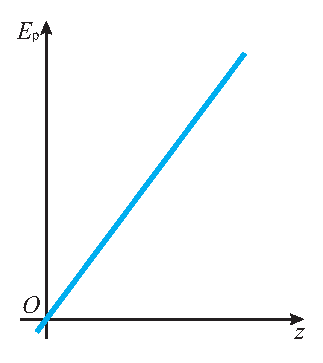
\includegraphics[width=\textwidth]{C3-kbfig3.1.eps}
		\caption{重力势能曲线}
		\label{C3-kbfig3.1}
	\end{subfigure}
	\begin{subfigure}[t]{0.4\textwidth}
		\centering
		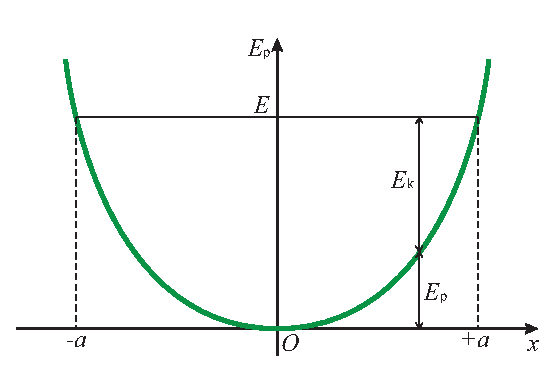
\includegraphics[width=\textwidth]{C3-kbfig3.3.eps}
		\caption{弹性势能曲线}
		\label{C3-kbfig3.3}
	\end{subfigure}
	\begin{subfigure}[t]{0.4\textwidth}
		\centering
		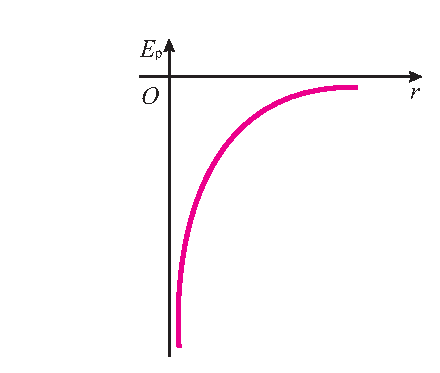
\includegraphics[width=\textwidth]{C3-kbfig3.2.eps}
		\caption{万有引力势能曲线}
		\label{C3-kbfig3.2}
	\end{subfigure}
	\caption{势能曲线}
\end{figure}

\subsection{机械能守恒定律}

\begin{enumerate}
	
	\item 质点机械能守恒定律
	
	\begin{equation}
		\dfrac{1}{2} m v_1^2 + E_{\mathrm{p1}} = \dfrac{1}{2} m v_2^2 + E_{\mathrm{p2}} \label{C3-eq21}
	\end{equation}
	
	\textbf{在仅有保守力做功时, 质点的动能和势能可以相互转换, 但动能和势能的总和保持不变. }
	
	\item 质点系机械能守恒定律
	
	\begin{equation}
		E_{\mathrm{k}} + E_{\mathrm{p}} = \text{Const} \label{C3-eq22}
	\end{equation}
	
\end{enumerate}

\section{能量守恒定律} \label{3.5}

\begin{axiom}[能量守恒定律] \label{C3-ax1}
	能量不能消失也不能创造, 只能从一种形式转化为另一种形式, 对于一个孤立系统来说, 不论发生何种变化, 各种形式的能量可以互相转换, 但它们的总和是一个常量. 
\end{axiom}

\section{第2次作业部分习题归纳} \label{3.6}

\subsection{做功}

\begin{enumerate}
	
	\item (作业T1) 如图(\ref{C3-fig1})所示,一个质点在几个力的作用下做半径为10 m的圆周运动,其中有一个力为$\va*{F} = 2 \va*{j}$ N, 则质点从$A$开始沿着逆时针方向经过半个圆周到达$B$点的过程中($AB$连线与$x$轴平行),该力做的功为 \uline{0}. 
	
\end{enumerate}

\subsection{动能}

\begin{enumerate}
	
	\item (作业T3) 质量为$m$的运动方程为$\va*{r} = A \cos \dfrac{2 \pi t}{T} \va*{i} + B \sin \dfrac{2 \pi t}{T} \va*{j}$, 式中$A$, $B$, $T$都是正的常量,则在$t = 0$到$t = \dfrac{T}{4}$这段时间内其动能的变化为 \uline{$2 m \pi^2 (A^2 - B^2) / T^2$}. 
	
\end{enumerate}

\begin{figure}[htbp]
	\centering
	\begin{subfigure}[t]{0.4\textwidth}
		\centering
		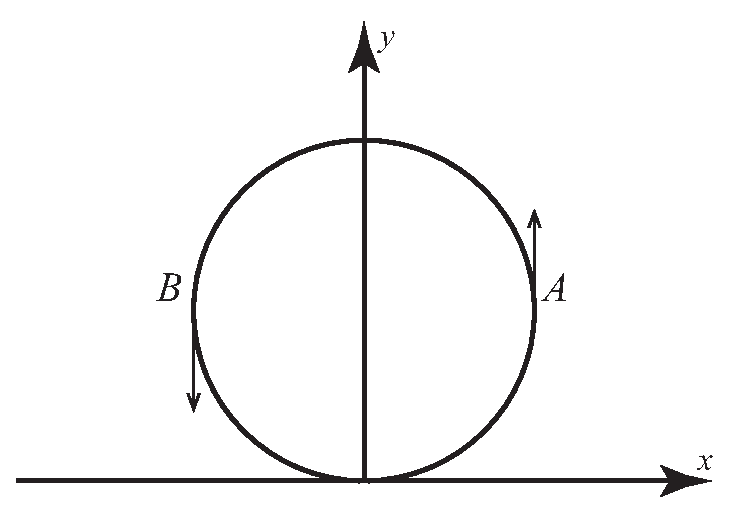
\includegraphics[width=\textwidth]{C3-fig1.eps}
		\caption{作业T1题图}
		\label{C3-fig1}
	\end{subfigure}
	\begin{subfigure}[t]{0.4\textwidth}
		\centering
		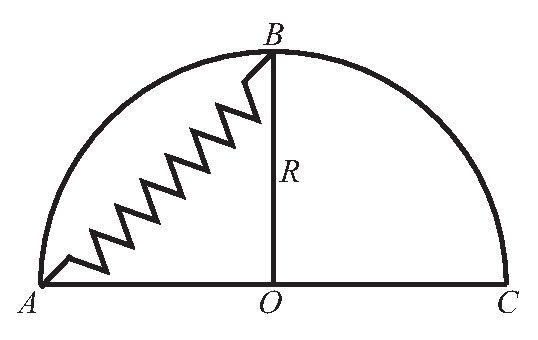
\includegraphics[width=\textwidth]{C3-fig2.eps}
		\caption{作业T20题图}
		\label{C3-fig2}
	\end{subfigure}
	\begin{subfigure}[t]{0.4\textwidth}
		\centering
		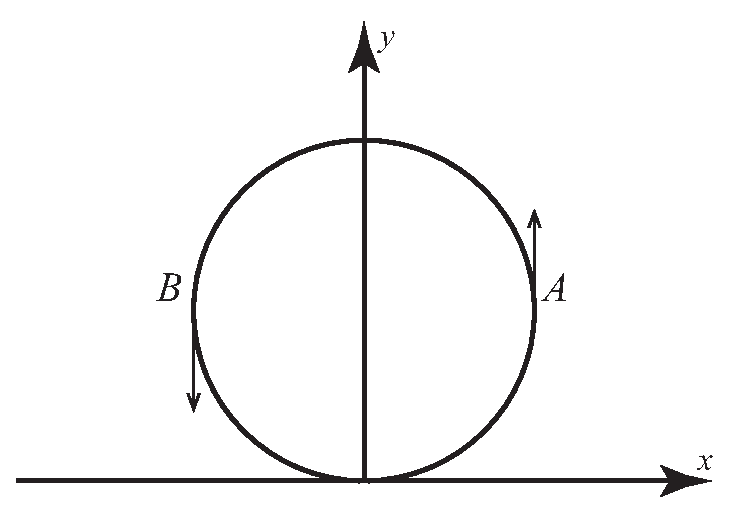
\includegraphics[width=\textwidth]{C3-fig1.eps}
		\caption{作业T18题图}
		\label{C3-fig3}
	\end{subfigure}
	\caption{3.6作业题图}
\end{figure}

\subsection{万有引力势能}

\begin{enumerate}
	
	\item (作业T19) 质量分别为$M$和$m$的两个质点,在万有引力的作用下,它们之间的距离由$r_1$缩短为$r_2$, 相应的万有引力所做的功为 \uline{$GMm(1/r_2 - 1/r_1)$}. 
	
\end{enumerate}

\subsection{弹性势能}

\begin{enumerate}
	
	\item (作业T20) 一弹簧原长$l_0 = 0.1$ m, 劲度系数$k = 40$ N/m, 其一端固定在半径为$R = 0.2$ m的半圆环端点$A$, 另一端与一套在半圆环上的小环相连, 如图(\ref{C3-fig2})所示.  在把小环由半圆环另一端$C$点移到半圆环中点$B$的过程中,弹簧的拉力对小环所作的功为 \uline{$4\sqrt{2}/5$ J}. 
	
\end{enumerate}

\subsection{动能定理}

\begin{enumerate}
	
	\item (作业T18) 几个船员站在静止的驳船上,船与人合计质量为 400 kg, 如图(\ref{C3-fig3})所示. 船员们用 200 N 的合力拉另一端系在岸边一树上的水平轻绳,则船开始运动后第2秒末的速率为 \uline{1 m/s}. 若不计水的阻力,那么在这段时间内,船和船员这一系统所增加的动能为 \uline{200 J}.
	
\end{enumerate}

\newpage
